\chapter{Models and Applications}
%\addcontentsline{toc}{chapter}{1 Graphs}
%%%%%%%%%%%%%%% SECTION HEADER %%%%%%%%%%%%%%%%
\rhead{3}
\lhead{Models and Applications}
%%%%%%%%%%%%%%%%%%% START %%%$%%%%%%%%%%%%%%%%%
\section{Word problems}
Word problems can be tricky. Often it takes a bit of practice to translate the English sentence into a mathematical sentence. This is what we will focus on here with some basic number problems, and simple interest problem.\\
A few important phrases are described below that can give us clues for how to set up a problem.
    \begin{table}[ht]
        \centering
        \caption{Conversion from English to math}
        \label{tbl:word}
        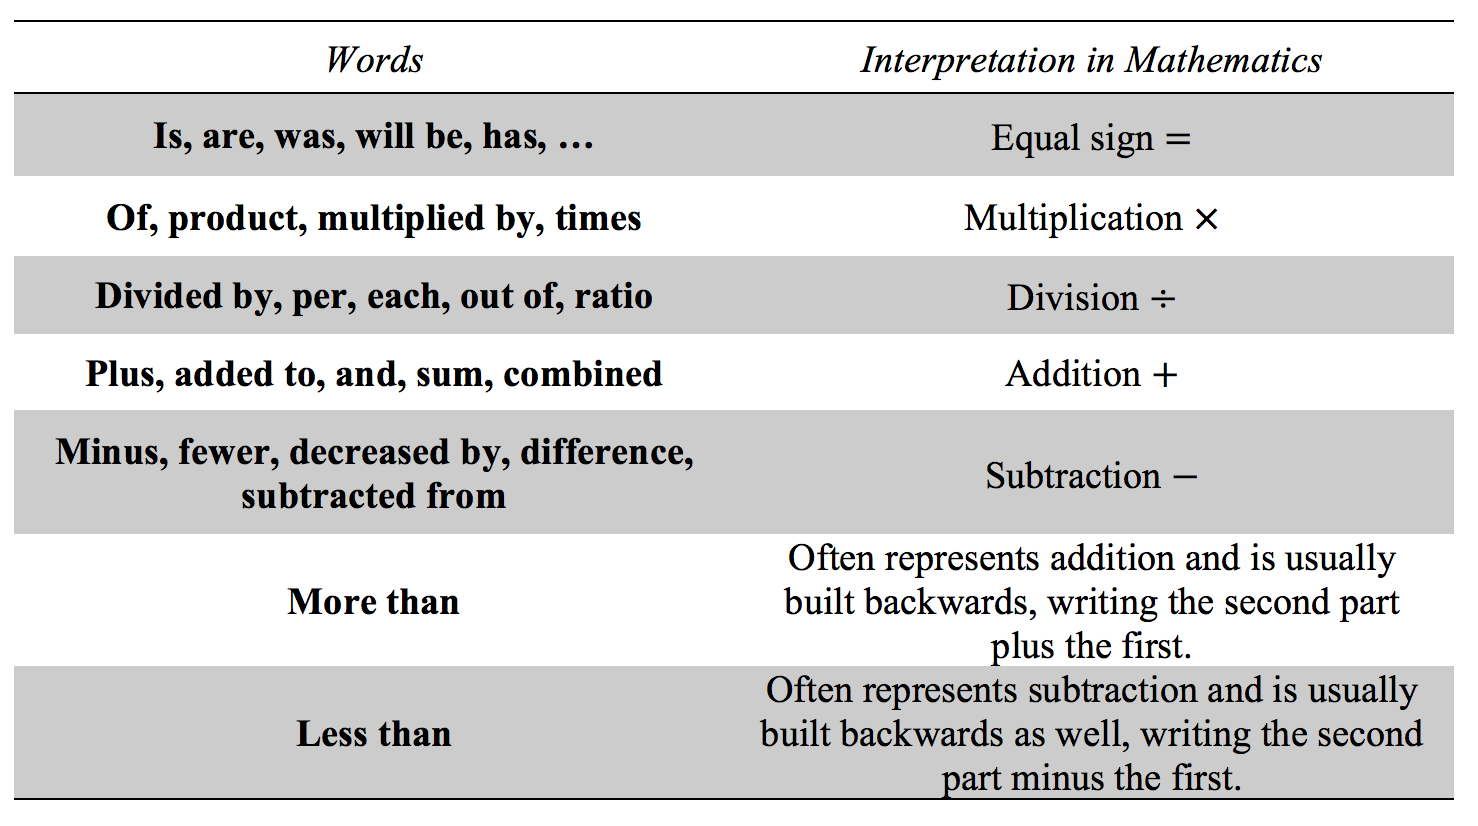
\includegraphics[width=12cm]{pics/word.png}
    \end{table}


Using these key phrases we can take a number problem and set up and equation and solve.
% ======== EXAMPLE 1
\begin{exa}
     If 25 less than five times a certain number is 235. What is the number?
\end{exa}
Let $x$ be the unknown number. Less than built backwards. we will have
\begin{gather*}
    \mathterm[a]{5}x\mathterm[b]{-}25\mathterm[c]{=} 235
\end{gather*}
\hspace*{2cm} five times\indicate{a}[out=0,in=-200]
\hspace*{0.2cm}  less than \indicate{b}[out=0,in=-90]
\hspace*{0.1cm}  is \indicate{c}[out=0,in=-60]

Now we can solve for $x$:
\begin{align*}
        5x-25 =235& &&\text{Add 25 to both sides}\\
        5x = 260&   &&\text{Divide by 5}\\
        x = 52& &&\text{The number is 52}
\end{align*}
% ========= EXAMPLE 2
\vspace{0.4cm}
\begin{exa}
     The average yearly salary of a woman with a bachelor's degree exceeds that of a woman with an associate's degree by $\$14$ thousand. The average yearly salary of a woman with a master's degree exceeds that of a woman with an associate's degree by $\$26$. Combined, three woman with each of these educational attainments earn $\$139$ thousand. Find the average yearly salary of woman with each of these levels of education.
\end{exa}
With no information about a woman with associate's degree, we call it $x$. Therefore
\begin{align*}
        x&  &   &\text{A woman with associate's degree}\\
     x+14&  &   &\text{A woman with bachelor's degree}\\
     x+26&  &   &\text{A woman with master's degree}
\end{align*}
We know three women combined earn $\$319$, thus
\begin{align*}
    x+(x+14)+(x+26) = 139&  &   &\text{This is our equation}\\
    3x+40 = 139&    &   &\text{Subtract 40 from both sides}\\
    3x = 99&   &   &\text{Divide both sides by 3}\\
    x = 33& &   &\text{Associate's degree}
\end{align*}
Thus, a bachelor will earn $x+14=33+14=47$ and one with master's degree will earn $x+26=33+26=59$.
% ============
\section{Simple interest}
When you borrow money from a bank or when a bank “borrows” your money by keeping it for you in a savings account, the borrower in each case must pay for the privilege of using the money. The fee that is paid is called interest. The most basic type of interest is simple interest, which is just an annual percentage of the total amount borrowed or deposited.\\
The amount of a loan or deposit is called the \textbf{principal $P$}. The annual percentage paid for the use of this money is the \textbf{interest rate $r$}. We will use the variable $t$ to stand for the number of years that the money is on deposit and the variable $I$ to stand for the total interest earned.
\begin{tcolorbox}[title=Simple Interest, 
                    fonttitle=\bfseries,
                    colframe=blue!70!red,
                    colback=white]
    The following simple interest formula gives the amount of interest $I$ earned:
    \begin{equation}
                I = Prt
                \label{simple_interest}
    \end{equation}
    where,
    \begin{itemize}
        \item $P$: principal (money deposited)
        \item $t$: years 
        \item $r$: interest rate (as a decimal)
    \end{itemize}
\end{tcolorbox}
%
\begin{nt}
    When using this formula, remember to convert $r$ from a percent to a decimal. For instance, in decimal form, 6\% is
    $\frac{6}{100}=0.06$.
\end{nt}
% =========== EXAMPLE 3
\begin{exa}
     You inherited $\$5000$ with the stipulation that for the first year the money had to be invested in two funds paying 9\% and 11\% annual interest. How much did you invest at each rate if the total interest earned for the year was $\$487$?
\end{exa}
The problem asks for the amount she has invested at each rate. So
we let \[
                x=\text{the amount invested at 9\%}
\]
Therefore, the remaining money invested at 11\% is
\[
            5000-x = \text{the amount invested at 11\%}
\]
The interest for each rate after 1 year can be found using the simple interest formula \eqref{simple_interest}
\begin{center}
\begin{tabular}{lcl}
    \toprule
    at 9\% rate   & &    at 11\% rate\\
    \hline 
    $I = x(0.09)(1)$ &  &    $I=(5000-x)(0.11)(1)$\\
    $\ \ \,= 0.09x$  & &  $\ \ \, =550-0.11x$ \\
    \bottomrule
\end{tabular}
\end{center}
Since the total interest was $\$487$ so
\begin{align*}
    \text{interest at 9\%} + \text{interest at 11\%} &= \text{total interest}\\
    0.09x + (550-0.11x) &= 487
\end{align*}
Now solve for $x$
\begin{align*}
        0.09x + (550-0.11x) = 487&   &   &\text{Combine like terms}\\
        550-0.02x=487&   &   &\text{Subtract 550 from both sides }\\
        -0.02x =-63& & &\text{Divide both sides by $-0.02$}\\
        x = 3150&   &   &\text{Invested at 9\%}
\end{align*}
For $11\%$, we invested $5000-x=5000-3150=1850$.
% ==============
\section{Solving a formula for on of its variable}
Solving formulas is like solving general linear equations except we will have several variables in the problem and we will be attempting to solve for one specific variable.\\
For example, let's consider \textit{Albert Einstein}'s famous formula $E=mc^2$. We may be interested in solving for the variable $m$. This means we want to isolate the $m$ so the equation has
$m$ on one side, and everything else on the other. So the solution looks like this $m=E/c^2$.\\
When solving formulas for a variable, we need to focus on the one variable we are trying to solve for, all the others are treated just like numbers.
% ====== EXAMPLE 4
\begin{exa}
     Solve the formula $P=2l+2w$ for $w$.
\end{exa}
We must isolate $w$
\begin{align*}
    P=2l+2w&    &   &\text{Subtract $2l$ from both sides}\\
    P-2l=2w&    &   &\text{Divide both sides by $w$}\\
    \frac{P-2l}{2}=w&   &   &\text{Our answer}
\end{align*}
% ========== EXAMPLE 5
\begin{exa}
     Solve the formula $P=C+MC$ for $C$.
\end{exa}
%
We need to isolate $C$
\begin{align*}
    P=C+MC&    &   &\text{Factor out $C$ on RHS}\\
    P=C(1+M)&    &   &\text{Divide both sides by $(1+M)$}\\
    \frac{P}{1+M}=C&   &   &\text{Our answer}
\end{align*}
% ========== EXAMPLE 6
\begin{exa}
     Solve the formula $\frac{1}{p}+\frac{1}{q}=\frac{1}{f}$ for $f$.
\end{exa}
Whenever you see a fraction, the first thing comes to your mind should be LCD. The LCD of $p$, $q$ and $f$ is $(pqf)$. 
\begin{align*}
    \frac{1}{p}+\frac{1}{q}=\frac{1}{f}&    &   &\text{Multiply both sides by LCD}\\
    %
    \textcolor{red}{pqf\biggl(}  \frac{1}{p}+\frac{1}{q}=\frac{1}{f} \textcolor{red}{\biggr)}&
    &&\text{Distribute}\\
    %
    \bcancel{p}qf\left(\frac{1}{\bcancel{p}}\right)+p\bcancel{q}f\left(\frac{1}{\bcancel{q}}\right)=pq\bcancel{f}\left(\frac{1}{\bcancel{f}}\right)&
    &&\text{Simplify}\\
    %
    qf+pf=pq&   &   &\text{Factor out $f$ on LHS}\\
    f(q+p)=pq&  &   &\text{Divide both sides by $q+p$}\\
    f = \frac{pq}{q+p}& &   &\text{Our answer}
\end{align*}